% !TEX root = ../gnss_interference_resistant_thesis.tex
\documentclass[main.tex]{subfiles}

\begin{document}

\subsection{GNSS signalų apdorojimas}

Signalų apdorojimui pasirinkta naudoti atviro kodo programinė įranga
GNSS-SDR \cite{GNSS-SDR11}. GNSS-SDR yra projektas, vystomas
Centre Tecnològic de Telecomunicacions de Catalunya organizacijos,
nuo 2011 metų.

GNSS signalų apdorojimas yra intensyvus procesas,
todėl norint apdoroti juos realiu laiku, reikalingos optimizacijos,
kurios pilnai išnaudotų kompiuterio resursus. Norint išnaudoti resursus,
visus skaičiavimus reikia lygiagretinti, tačiau tai nėra tokia
paprasta užduotis. Ši problema jau yra išspręsta GNU Radio projekto,
todėl GNSS-SDR pasitelkia šį įrankį signalų apdorojimui.

\begin{figure}[h]
    \begin{centering}
    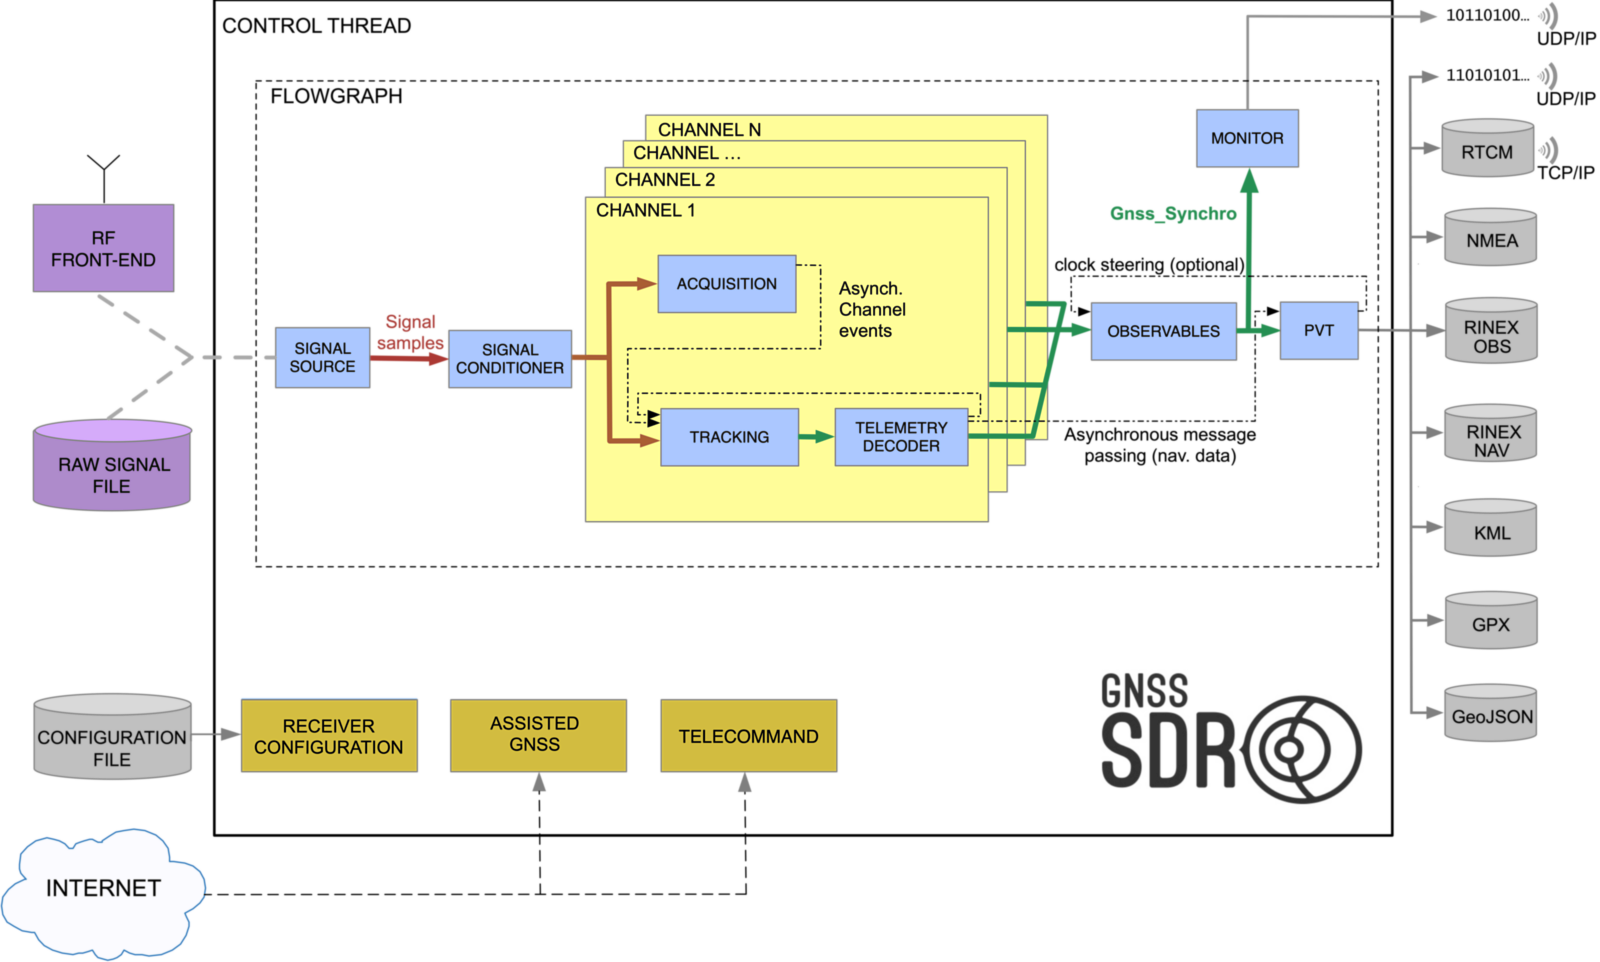
\includegraphics[scale=12.0]{drawings/GeneralBlockDiagram}
    \par\end{centering}
    \protect\caption{\label{fig:gnss_sdr_block}GNSS SDR imtuvo, duomenų apdorojimo schema \cite{gnss_sdr_web}.}
\end{figure}

Signalo apdorojimas prasideda nuo duomenų šaltinio (angl. Signal Source). Duomenų šaltiniu
gali būti arba SDR imtuvas, arba duomenų failas. Dažniausiai SDR imtuvas naudojamas,
kai duomenys yra apdorojami realiu laiku, o duomenų failas, kai duomenys yra apdorojami
vėliau, taip pat duomenų failas yra patogesnis naudojimui, kai yra tobulinamas GNSS SDR
programinis kodas, kadangi galima nesunkiai lyginti imtuvo kokybę su tuo pačiu signalu.

Duomenys iš šaltinio turi būti pritaikyti prie vidinio formato. Signalo šaltiniai
dažnai turi skirtingus formatus, skiriasi duomenų rezoliucija, išdėliojimas ir t.t.
Signalo paruošimo (angl. Signal Conditioner) paskirtis yra pritaikyti duomenų šaltinio
formatą prie vidinio formato, naudojamo visuose kituose apdorojimo blokuose.

Kanalai (angl. Channel) yra skirti individualių palydovų paieškai ir sekimui.
Kiekvienas kanalas yra atsakingas už palydovo signalo suradimą (angl. Acquisition),
jį suradus, už jo signalo sekimą (angl. Tracking) ir duomenų dekodavimą (angl. Telemetry
Decoder). Visi kanalai veikia lygiagrečiai, iš pradžių kiekvienam kanalui yra
priskiriamas palydovas kurio jis ieškos ir tada pradedama palydovų paieška.
Aptikus palydovo signalą, pradiniai sekimo parametrai yra perduodami sekimo
blokui, kuris užsirakina ant signalo.

Stebėjimo blokas (angl. Observables) surenka duomenis iš visų kanalų ir atlieka
pseudo atstumo, fazės ir Doplerio dažnio matavimus. Iš šių duomenų, galime
rasti imtuvo poziciją, greitį ir laiką, už tai yra atsakingas PVT
(angl. Position-Velocity-Time) blokas. Šis blokas atsakingas už sprendinio
radimą ir rezultato pateikimą skirtingais standartizuotais formatais.

\subsubsection{GNSS signalo sekimo blokas}\label{sec:tracking_block}

Sekimo bloko pagrindinė užduotis yra sekti signalo sinchronizacijos parametrus:
kodo užlaikymą ($\tau(t)$), Doplerio dažnį ($f_D(t)$) ir nešlio fazę ($\phi(t)$).

Pasinaudojus didžiausio tikėtinumo metodas (ML), bandoma maksimizuoti priimamo
signalo koreliaciją su lokaliai atkurtu signalu. ML sekami parametrai $f_D$ ir
$\tau$ gali būti surasti maksimizuojant šią funkciją:

\begin{equation}
    \hat{f}_{D_{ML}},\hat{\tau}_{ML} = \arg \max \left\{ \left| \hat{R}_{xd}(f_D, \tau) \right|^2 \right\},
\end{equation}

\noindent kur

\begin{equation}
    \hat{R}_{xd}(f_D, \tau) = \frac{1}{K} \sum^{K-1}_{k=0} {x_{IN}[k]d[kT_s-\tau]e^{-j2\pi f_D kT_s}},
\end{equation}

\noindent čia $x_{IN}[k]$ signalas aprašytas \refeq{eq:gps_signal}, $d[k]$ - lokali palydovo
signalo kopija, $K$ - taškų skaičius naudojamas koreliacijai.

Signalo sekimas yra pasiekiamas pasinaudojus uždaro kontūro sistemomis,
kurios yra su\-pro\-jek\-tuo\-tos taip, kad minimizuotų skirtumus tarp kodo užlaikymo,
Doplerio dažnio ir nešlio fazės lyginant su lokalia signalo kopija $d[k]$.

GNSS signalų atveju imtuvas skaičiuoja 3-jų signalų $R_{xd}$ koreliacijas:
paankstinto signalo $E=R_{xd}(\hat{\tau} + \epsilon)$,
tikrasis signalas $P=R_{xd}(\hat{\tau})$,
pavėlintas signalas $L=R_{xd}(\hat{\tau} - \epsilon)$.
Atlikus koreliacijas, palyginami rezultatai ir taip nustatoma
ar lokali signalo kopija atsilieka, skuba, ar tiksliai atkartoja
priimamą signalą. Atlikus skaičiavimus atnaujinama lokali signalo kopija
ir vėl viskas vykdoma iš naujo. Signalo sekimo blokinė diagrama pavaizduota
\ref{fig:gnss_sdr_tracking_block}~pav.

\begin{figure}[h]
    \begin{centering}
    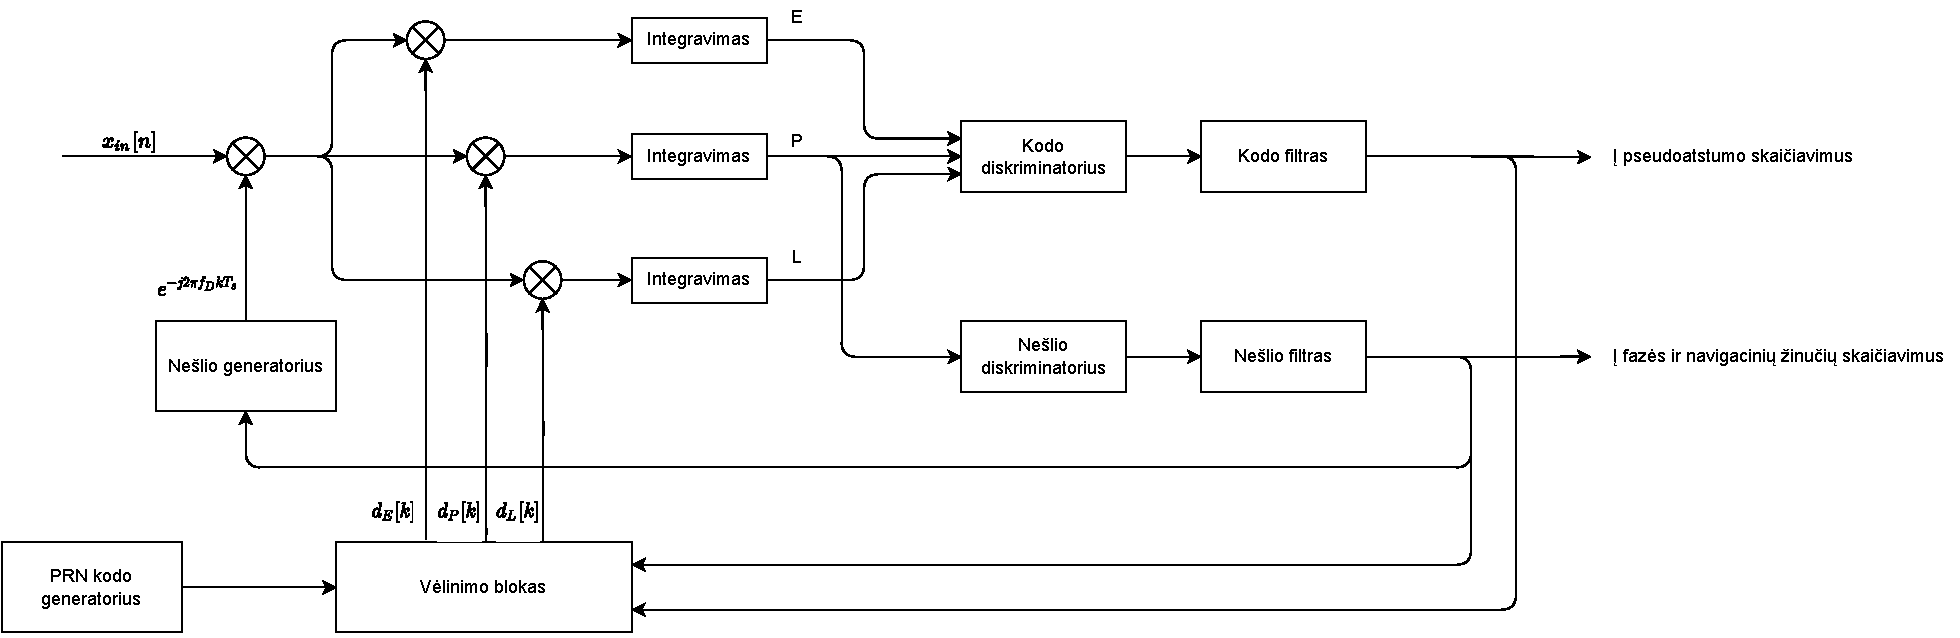
\includegraphics[scale=0.5]{drawings/tracking_diagram}
    \par\end{centering}
    \protect\caption{\label{fig:gnss_sdr_tracking_block}GNSS signalo sekimo blokinė diagrama \cite{gnss_sdr_web}.}
\end{figure}

\subsubsection{GNSS signalo ir triukšmo santykio nustatymas}\label{sec:gnss_snr}

Signalo ir triukšmo tankio santykis gali būti išreikštas kaip $C/N_0 = \frac{C}{\frac{N}{BW}}$,
kur $C$ yra nešlio galia, $N$ - triukšmų galia, $BW$ - imtuvo juostos plotis.
Ši išraiška parodo nešlio galios ir triukšmo galios santykį per juostos pločio vienetą.
Santykis $\frac{C}{N}$ vadinamas signalo triukšmo santykiu (SNR).

Laikant, kad dažnių juostos plotis yra atvirkščiai proporcingas integravimo laikui $T_{int}$,
galime užrašyti:

\begin{equation}
    C/N_0 = \frac{SNR}{T_{int}}.
    \label{eq:snr_integration}
\end{equation}

Kompleksiniams skaičiams SNR gali būti suskaičiuotas pasinaudojus antro ir ketvirto
laipsnio momentų vertintoju \cite{871393}:

\begin{equation}
    \widehat{SNR} = \frac{\hat{C}}{\hat{N}} = \frac{\sqrt{2 \hat{\mathcal{M}}_2^2 - \hat{\mathcal{M}}_4 }}{\hat{\mathcal{M}}_2 - \sqrt{2 \hat{\mathcal{M}}_2^2 - \hat{\mathcal{M}}_4 }}~,
    \label{eq:snr_moment}
\end{equation}

\noindent čia:
\begin{itemize}
    \item $\hat{\mathcal{M}}_2 = \frac{1}{M} \sum^{M-1}_{m=0}{\left| P[m] \right|^2}$, 
    \item $\hat{\mathcal{M}}_4 = \frac{1}{M} \sum^{M-1}_{m=0}{\left| P[m] \right|^4}$,
    \item $M$ - taškų skaičius naudojamas SNR įvertinimui,
    \item $P[m]$ - nevėlinto koreliatoriaus kompleksinė vertė (aprašyta \ref{sec:tracking_block} skyriuje).
\end{itemize}

Pasinaudojus \refeq{eq:snr_integration} ir \refeq{eq:snr_moment} galime išreikšti
$C/N_0$ vertę $\mathrm{dB-Hz}$ vienetais:

\begin{equation}
    \widehat{C/N}_{0_{dB-Hz}} = 10\log_{10}(\widehat{SNR})-10\log_{10}(T_{int})~.
\end{equation}


\end{document}
